%%%%%%%%%%%%%%%%%%
%%%%%% RFKO %%%%%%
%%%%%%%%%%%%%%%%%%
\subsection{Slow extraction - RFKO}

The ion slow extraction scheme uses the magnetic septums SMH57 and SMH61 to extract the beam to the East Area. Unlike the proton slow extraction, in the case of the lead ion beam, the electrostatic septum SEH23 is bypassed as its entry and exit windows would strip the ions from the remaining electrons, which would change the rigidity during extraction; see Fig. \ref{fig:sx}.

\begin{figure}[!htb]
\centering
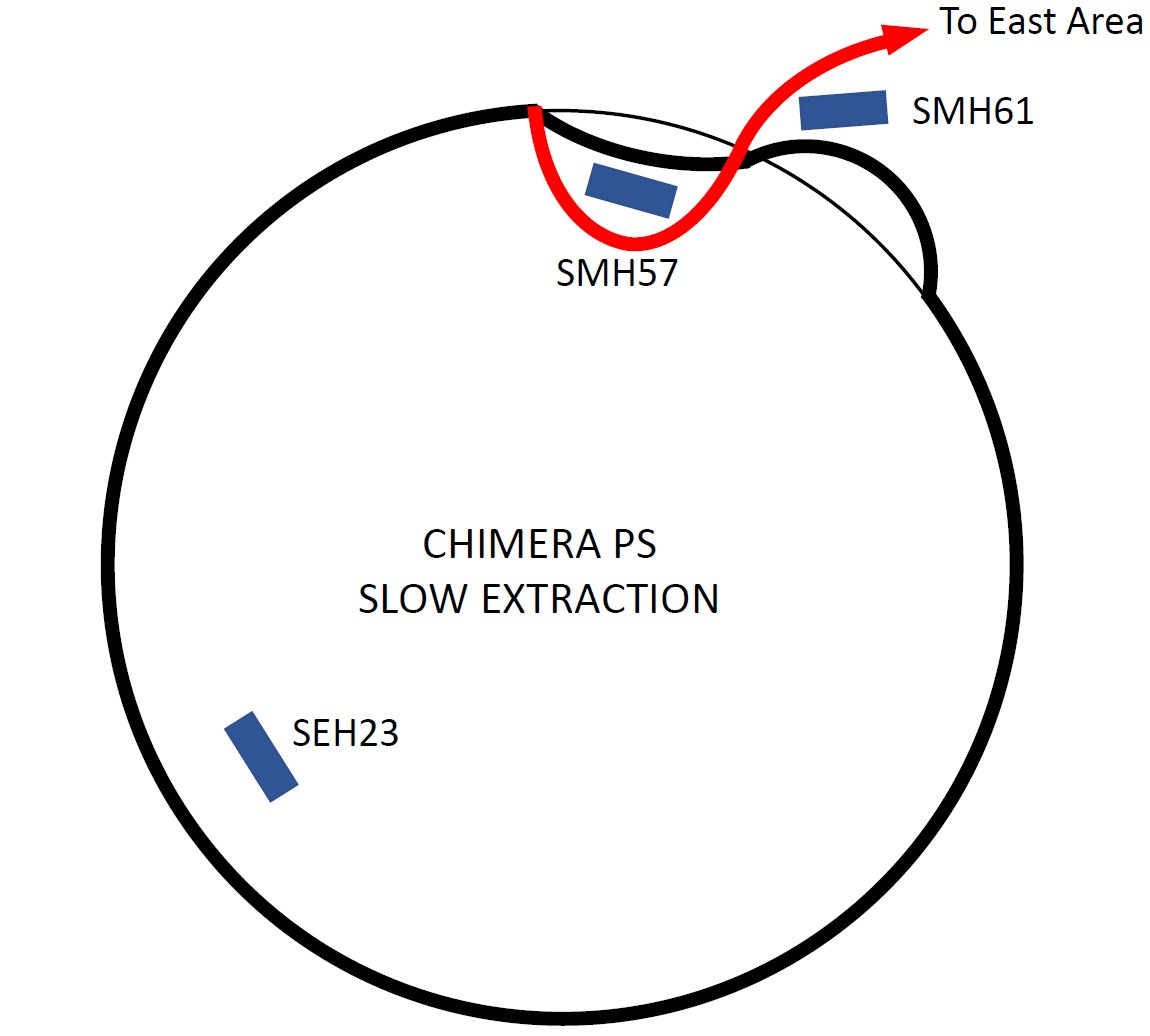
\includegraphics[width=0.4\textwidth]{images/BEAM_INTENSITY/SX_CHIMERA.jpg}
\caption{Pb-ion beam slow extraction scheme}
\label{fig:sx}
\end{figure}

To jump the septum, the required amplitude growth is achieved through the use of bumps and third-order integer slow extraction. The standard slow extraction technique in the PS involves shrinking a third-order integer triangle formed by separatrices (produced by a non-linear field) by changing the horizontal betatron tune (Qx). Iterations of the scheme were performed, beginning with a ramp on the low-energy quadrupoles (LEQ) to increase the tune to the third integer resonant tune. However, a different slow extraction scheme using Radiofrequency Knock Out (RFKO) was ultimately adopted during the 2022 November run to improve the control of the beam intensity at different energies. In RFKO, the beam is slowly extracted due to emittance growth induced by a transverse RF-field at a third of the revolution frequency. The resonance line serves as a threshold above which the particles become unstable. The RF-frequency is modulated over time (using frequency modulation, or FM, close to a third of the revolution frequency), with a frequency sweep (or chirp) performed to affect off-momentum particles. The chirping signal increases the beam emittance and diffuses the particles from the beam core to the stable triangle, see Fig. \ref{fig:steinbach_diagram} and \ref{fig:rfko}. The frequency sweep ensures that a large fraction of the particles in the beam are kicked and start the diffusion process. As the machine does not ramp, the stable triangle remains fixed in phase-space during the extraction \cite{noda_slow_1996, badano_proton-ion_1999, dulla_radio_2019}.
\\

\begin{figure}
    \centering
    \begin{minipage}{0.45\textwidth}
        \centering
        \begin{tikzpicture}
            \path [fill=lightgray] (1,0) -- (-6,3) -- (2,3) -- (2,1) -- (1,0);
        	\draw [->, thick] (-6,0) -- (2,0) node [below left] {\small$\Delta p/p$};
        	\draw [->, thick] (0,0) -- (0,4)  node [below left] {Amplitude (V)};
         % Waiting stack
            \draw[fill=gray] (-4,0) rectangle (-3.5,2);
         % Extracted beam
            \fill[fill=white, fill opacity=0.9] (-4,2) rectangle (-3.5,3);
            \fill[fill=gray, fill opacity=1.0, pattern = crosshatch dots] (-4,2) rectangle (-3.5,3);
        \draw [->, line width = 1mm] (-3.75,2.2) -- (-3.75,2.8);
        \end{tikzpicture} 
        \caption{In RFKO, transverse stochastic noise or RF excitation at the revolution frequency is used to excite the beam and induce growth in its betatron amplitudes.}
        \label{fig:steinbach_diagram}
    \end{minipage}\hfill
    \begin{minipage}{0.45\textwidth}
        \centering
        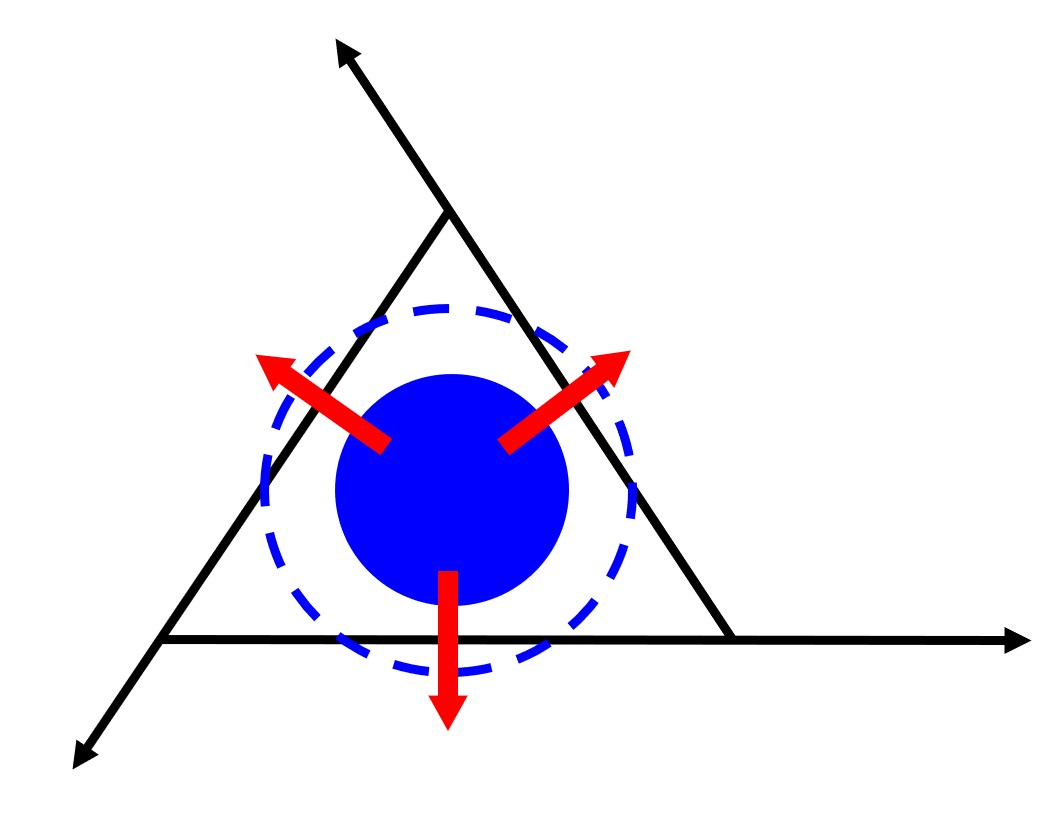
\includegraphics[width=1.0\textwidth]{images/BEAM_INTENSITY/RFKO.jpg}
        \caption{The emittance growth diffuses the particles from the beam core to the unstable triangle.}
        \label{fig:rfko}
    \end{minipage}
\end{figure}

The RFKO setup involved using the radial loop GRPOS to bring the beam's tune close to resonance, followed by a slight backing off from the resonance using the same radial loop. This was preferred over using the low-energy quadrupoles (LEQ), which also changes the tune but also the optics. Once the target tune was attained, the radial loop was turned off and the beam was debunched. The optics of the machine remained static, without any ramping. The Transverse Feedback Blowup (TFB) was then employed to push particles into resonance with the help of the the Q-meter software to chirp the beam. At low frequencies, the chirps were visible in the spill, but for faster chirping $< 1$ ms, the frequencies were high enough to be mostly suppressed by the transit time. For more details on the beam time structure, see section \ref{beam_time_structure}.

%%%%%%%%%%%%%%%%%%%%%%%%%%%%
%%%%%% BEAM INTENSITY %%%%%%
%%%%%%%%%%%%%%%%%%%%%%%%%%%%
\subsection{Beam intensity}
\label{beam_intensity}



The RFKO scheme has different parameters to control the extraction:
\begin{enumerate}
    \item Chirp gain: the voltage applied to the RFKO plates.
    \item Chirp frequency range
    \item Accuracy (number of turns in the PS)
    \item Bounds: Start and stop of the chirping
\end{enumerate}

Lowest chirps is 512 turns
Time it takes for one turn in the PS = **2.1 $\mu s$**
* $t = \frac{circumference}{c} = \frac{628}{3e8} = 2.1e-6 [s]$

5.12e2 * 2.1e-6 = 1.752e-3 s = 1.8 ms

\begin{figure}[!htb]
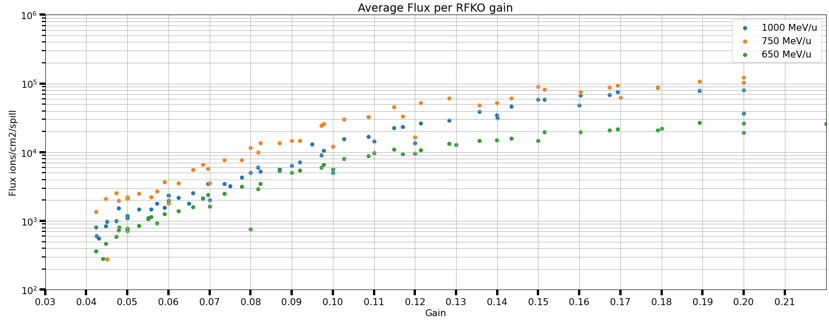
\includegraphics[width=1.0\textwidth]{images/BEAM_INTENSITY/flux_vs_gain.png}
\end{figure}


Additionally, the smallest beam area with the constraints on power converter amperage of 733, 537 and 421 A respectively is simulated to be 0.904 mm.

